\documentclass[11pt]{article}  
\usepackage{a4wide,ngerman,url,amsmath,bbm,graphicx,enumitem}
\usepackage[utf8]{inputenc}

\newcommand{\br}[1]{\ensuremath{\left(#1\right)}}
\newcommand{\cbr}[1]{\ensuremath{\left\{#1\right\}}}
\newcommand{\ii}{\mathrm{i}}
\newcommand{\N}{\mathbbm{N}}
\newcommand{\Z}{\mathbbm{Z}}
\newcommand{\ggT}{\mathrm{ggT}}
\newcommand{\HGG}[1]{\begin{quote} Einfügen: #1 \end{quote}}
\def\pw{{\char94}}

\newenvironment{code}{\tt \begin{tabbing}
\hskip12pt\=\hskip12pt\=\hskip12pt\=\hskip12pt\=\hskip5cm\=\hskip5cm\=\kill}
{\end{tabbing}}

\parindent0pt
\parskip3pt

\author{Bernd Winter, Korrekturen durch Hans-Gert Gräbe}
\title{Zur Konstruktion regulärer Polygone, insbesondere des regulären
  17-Ecks, 257-Ecks und 65537-Ecks} 
\date{Erstellt 2012, letztes Update 06.12.2020}

\begin{document} 
\maketitle         
\begin{quote}
  Quelle: \url{https://www.mathematik-olympiaden.de/moev/moev_material/}\\
  \url{Konstruktion17/index.html}

  Dort auch ein Video zur Konstruktion des regulären 257-Ecks, Impressionen
  zum legendären Koffer mit der Arbeit zum 65537-Eck von \textsc{Hermes} in
  Göttingen.
\end{quote}
Reguläre Polygone oder $n$-Ecke sind solche $n$-Ecke mit gleicher Seitenlänge
$a_n$.  Die klassischen Konstruktionswerkzeuge nach \textsc{Euklid} (etwa 365
v. Chr. bis etwa 300 v. Chr.) sind Zirkel und Lineal (ohne Messfunktion).
Damit können Kreise um einen (Mittel)punkt durch einen zweiten Punkt, Geraden,
Strahlen und Strecken durch zwei Punkte, Schnittpunkte zweier Kreise, zweier
Geraden oder zwischen Kreis und Gerade (Strahl oder Strecke) konstruiert
werden.

Wenn man ein $x$-$y$-Koordinatensystem in der Zeichenebene einführt, kann man
z. B. Kreise mittels der Gleichung $\br{x-x_m}^2+\br{y-y_m}^2=r^2$ ($x_m$,
$y_m$ Koordinaten des Kreismittelpunkts, $r$ Kreisradius) oder Geraden mittels
der Gleichung $ax + by = c$, ($a \neq 0$ oder $b \neq 0$) darstellen.
Schnittpunkte dieser Objekte lassen sich mit Gleichungssystemen aus derartigen
Gleichungen oder Folgen derartigen Gleichungssysteme beschreiben. (Es kommen
also z. B. keine Gleichungen dritten Grades vor.) Die Lösungen derartiger
Systeme, sofern diese existieren, sind also endlich lange Terme, die reelle
Zahlen, evtl. verknüpft durch die vier Grundrechenarten und Quadratwurzeln
sowie Verschachtelungen davon enthalten. (Siehe z. B. den Ausdruck (1)).

Größtenteils bereits seit dem Altertum (\textsc{Euklid}) sind Konstruktionen
mit Zirkel und Lineal u. a. für einige reguläre $n$-Ecke bekannt, insbesondere
für das reguläre 3-, 4- und 5-Eck: Man erkennt sofort die „Verwandtschaft“ der
regulären $n$-Ecke in den „Familien“ der regulären 3-, 6-, 12-, 24-, ... -Ecke
oder der 4-, 8-, 16-, ... -Ecke oder der 5-, 10-, 20-, ... -Ecke.

Durch geschickte Kombination ließen sich z. B. auch reguläre 15-Ecke
konstruieren: Nach dem Lemma von \textsc{Bézout} (1730--1783) gibt es für zwei
natürliche Zahlen $a$ und $b$, hier 3 und 5, zwei ganze Zahlen $s$ und $t$, so
dass sich der größte gemeinsame Teiler $\mathrm{ggT}(a,b)$ der Zahlen $a$ und
$b$ als $\ggT(a,b) = s \cdot a + t \cdot b$ darstellen lässt. Da Primzahlen
und somit auch \textsc{Fermat}sche Primzahlen stets teilerfremd zueinander
sind, ist $\ggT(3,5) = 1$. So ist $1 = s \cdot 3 + t \cdot 5$. Man kann die
Zahlen $s$ und $t$ mit dem erweiterten \textsc{Euklid}ischen Algorithmus
bestimmen:
\begin{align*}  
  5 : 3 &= 1\ \text{Rest}\ 2 & 	2 &= 5 - 1 \cdot 3\\{}
  3 : 2 &= 1\ \text{Rest}\ 1 &	1 &= 3 - 1 \cdot 2\\{}
  && 1 &= 3 - 1 \cdot (5 - 1 \cdot 3)\\{}
  && 1 &= 2 \cdot 3 - 1 \cdot 5
\end{align*}
So ist $s = +2$ und $t = -1$.

Anschaulich ausgedrückt heißt das: Man zeichne den (Bestimmungs)winkel
($72^\circ$) des regulären 5-Ecks im mathematisch positiven Drehsinn (gegen
den Uhrzeigersinn) und füge einen weiteren Winkel mit dieser Größe an. Man
füge in entgegengesetztem Drehsinn den (Bestimmungs)winkel ($120^\circ$) des
regulären 3-Ecks an. Der Gesamtwinkel ist der Bestimmungswinkel des regulären
15-Ecks.

\HGG{Animiertes gif images/15-Eck.gif hier einbinden}

Sofort fällt auf, dass in diesen Mengen u. a. das reguläre 7-, 9- und 17-Eck
nicht enthalten sind. Bis zum Ende des 18. Jahrhunderts war die Frage der
Konstruierbarkeit dieser regulären $n$-Ecke ungelöst.

\textsc{Gauss} (1777-1855) konnte dieses Problem lösen. Er schrieb 1819 dazu:
„Die Geschichte jener Entdeckung ist bisher nirgends von mir öffentlich
erwähnt, ich kann es aber sehr genau angeben. Der Tag war der 29. März
1796\footnote{\textsc{Gauss} gibt in diesem Brief den 30. März als Tag seiner
  Entdeckung der Kreisteilung an, ein Tag später als in der zitierten Aussage
  \cite[S. 219]{Paucker1822}.}, und der Zufall hatte gar keinen Anteil
daran. Schon früher war alles ... von mir gefunden ..., und zwar im Winter
1796 (meinem ersten Semester in Göttingen), ohne daß ich den Tag aufgezeichnet
hätte. Durch angestrengtes Nachdenken über den Zusammenhang aller Wurzeln
(heutiger Begriff: Lösungen -- d. A.)  untereinander nach arithmetischen
Gründen glückte es mir, bei einem Ferienaufenthalt in Braunschweig am Morgen
des gedachten Tages (ehe ich aus dem Bette aufgestanden war) diesen
Zusammenhang auf das klarste anzuschauen, so daß ich die spezielle Anwendung
auf das 17-Eck und die numerische Bestätigung auf der Stelle machen konnte.“
(\cite[S. 15\,f]{GaussTagebuch}, sinnwahrend vom Autor gekürzt.)

Der im Text beschriebene Ausdruck ist: 
\begin{align*}
  \cos\br{\frac{2\pi}{17}}&= \frac{1}{16}
  \Bigg(-1+\sqrt{17}+\sqrt{{2\br{17-\sqrt{17}}}}+\\ &\qquad
  2\sqrt{17+3\sqrt{17}-\sqrt{2\br{17-\sqrt{17}}}-2\sqrt{2\br{17+\sqrt{17}}}}
  \Bigg) \tag{1}
\end{align*}

Es sei auf die ausführliche lesenswerte Herleitung der Gleichung durch
Patzschke \cite{Patzschke2002} verwiesen. Der Winkel $\frac{2\pi}{17}$ ist der
in Bogenmaß ausgedrückte Bestimmungswinkel des regulären 17-Ecks.

Ausführlich hat \textsc{Gauss} seine Theorie in seinem Werk „Disquisitiones
arithmeticae“ 1801 dargestellt: Ausgangspunkt ist die Vorstellung, dass die
Konstruktion des regulären $n$-Ecks im Einheitskreis äquivalent zur Bestimmung
der Lösungen der Kreisteilunggleichung $x^n - 1 = 0$ ($n\in\N$) ist.

Er fand dann die hinreichende Bedingung für die Konstruktion regelmäßiger
Polygone. Er vermutete, dass die Bedingung auch notwendig ist, gab allerdings
keinen Beweis an. \textsc{Wantzel} (1814-1848) holte dies 1837
nach\footnote{\url{http://de.wikipedia.org/wiki/Wantzel} (abgerufen am
  01.09.2011).}.

Diese notwendige und hinreichende Bedingung für die Konstruierbarkeit des
regulären $n$-Ecks an die Zahl $n$ lautet:
\begin{quote}
  $n$ ist eine natürliche Zahl größer als 2 und $n$ ist ein Produkt aus einer
  Potenz von 2 mit einer nichtnegativen ganzen Zahl als Exponenten und
  möglicherweise als weitere Faktoren voneinander verschiedene FERMATsche
  Primzahlen.
\end{quote}
Diese speziellen Primzahlen sind nach dem französischen Mathematiker und
Juristen \textsc{Fermat} (1601--1665) benannt.

Potenzen von 2 sind 4, 8, 16, ...

Man erkennt auch sofort die oben genannten „Familien“ konstruierbarer
regulärer $n$-Ecke wieder.

\textsc{Fermat}sche Primzahlen $n =2^{\br{2^k}}, k\in\N$.
\begin{align*}
  k = 0 &\rightarrow{} n = 3\\
  k = 1 &\rightarrow{} n = 5\\
  k = 2 &\rightarrow{} n = 17\\
  k = 3 &\rightarrow{} n = 257\\
  k = 4 &\rightarrow{} n = 65537
\end{align*}
Bis jetzt sind keine weiteren \textsc{Fermat}schen Primzahlen gefunden
worden\footnote{\url{http://de.wikipedia.org/wiki/Fermat-Zahl} (abgerufen am
  16.05.2012).}.

Sollte es so sein, dass es genau diese fünf \textsc{Fermat}schen Primzahlen
gibt, so folgt daraus unmittelbar, dass nur 31 (= $2^5 - 1$) regelmäßige
Polygone mit ungerader Eckenzahl mit Zirkel und Lineal konstruierbar
sind. Sollte es weitere \textsc{Fermat}sche Primzahlen, aber insgesamt nur
endlich viele, geben, so bliebe die Anzahl mit Zirkel und Lineal
konstruierbarer regelmäßiger $n$-Ecke mit ungeradem $n$ auch endlich. Diese
Anzahl ist $2^m - 1$, dabei sei $m$ die Anzahl der \textsc{Fermat}schen
Primzahlen.

Nun war klar, dass das reguläre 17-Eck, aber auch das reguläre 257-Eck und das
reguläre 65537-Eck mit Zirkel und Lineal konstruierbar sind (siehe unten).
Somit waren die bekannten Konstruktionen theoretisch untermauert und es konnte
über die praktische Umsetzung der Konstruierbarkeit weiterer regulärer
$n$-Ecke nachgedacht werden.

Besonders bemerkenswert ist die Verknüpfung verschiedener Teilgebiete der
Mathematik durch \textsc{Gauss}: Das Problem war geometrischer Natur, die
Lösung des Problems wurde über den Weg der Analysis in der Algebra
gefunden. Rund 200 Jahre später noch einmal ein noch genialerer mathematischer
„Coup“: Der Beweis des Großen \textsc{Fermat}schen Satzes durch \textsc{Wiles}
1995\footnote{\url{http://de.wikipedia.org/wiki/Großer_Fermatscher_Satz}
  (abgerufen am 16.05.2012)}. Auch hierbei wurden mit noch weitaus größerem
Aufwand Erkenntnisse verschiedener mathematischer Gebiete verbunden, um zum
gewünschten Beweis zu kommen.

Die zentrale Rolle des Bestimmungswinkels bzw. seines Kosinus zur Konstruktion
des zugehörigen regulären Polygons ist in der folgenden Abbildung am Beispiel
des regulären Achtecks zu sehen: 
\begin{itemize}
\item Konstruiere Einheitskreis.
\item Konstruiere Strecke der Länge $\cos\br{\alpha=\frac{2\pi}{n}}$.
\item Konstruiere Parallele zur $y$-Achse.
\item Konstruiere Bestimmungsdreieck des regulären $n$-Ecks.
\item Konstruiere das Polygon.
\end{itemize}

\HGG{Animation der Konstruktion des regelmäßigen Achtecks einfügen}

Einige Beispiele dafür:
\begin{align*}  
  &\cos\br{\frac{2\pi}{3}}=\frac{1}{2},\\
  &\cos\br{\frac{2\pi}{5}}=\frac{1}{2}\br{-1+\sqrt{5}}.
\end{align*}
Eine Darstellung von $\cos\br{\frac{2\pi}{7}}$ in ähnlicher Form als endlich
langer Term, bestehend aus reellen Zahlen, evtl. verknüpft durch die vier
Grundrechenarten und Quadratwurzeln sowie Verschachtelungen davon, ist nicht
möglich (siehe oben).
\begin{align*}
  \cos\br{\frac{2\pi}{17}}&= \frac{1}{16}
  \Bigg(-1+\sqrt{17}+\sqrt{{2\br{17-\sqrt{17}}}}+\\ &\qquad
  2\sqrt{17+3\sqrt{17}-\sqrt{2\br{17-\sqrt{17}}}
    -2\sqrt{2\br{17+\sqrt{17}}}}\Bigg)
\end{align*}
Ein mit \textsc{Mathematica} Version 5.2 erstellter symbolischer Ausdruck von
$\cos(2\pi/257)$ (pdf-Datei \texttt{cos2pi\_257\_symbolisch.pdf}, etwa 640
KByte) sei nach Auskunft des Softwareherstellers durch einen Bug fehlerhaft.
Eine Umwandlung von $\cos\br{\frac{2\pi}{257}}$ in einen symbolischen Ausdruck
mit verschachtelten Quadratwurzeln erfolgt in neueren Versionen nicht mehr. Es
wird nur die Äquivalenz
\begin{gather*}
  \cos\br{\frac{2\pi}{257}}= -\frac{1}{2}\br{\br{-1}^{\frac{255}{257}}\cdot
    \br{1+\br{-1}^{\frac{4}{257}}}}
\end{gather*}
ausgegeben.

Es gibt auch einen interessanten Bezug zur Graphentheorie. Um ein reguläres
Polygon zu konstruieren, reicht es, wie oben beschrieben, wenn man den
Bestimmungswinkel des regulären $n$-Ecks kennt. Dieser ergibt sich, wenn man
neben einem frei wählbaren Eckpunkt, sozusagen einem trivialen Eckpunkt, einen
weiteren benachbarten Eckpunkt kennt. Somit sind dann alle Eckpunkte
konstruierbar. Das bedeutet, es sind, wenn die Eckenanzahl $n$ eine
\textsc{Fermat}sche Primzahl ist, also eine der Zahlen 
\begin{gather*}
  5-1=4=2^2, 17-1=16=2^4, 257-1=256=2^8\ \text{oder}\ 65537-1=65536=2^{16},
\end{gather*}
entsprechende „nichttriviale“ Eckpunkte zu konstruieren. Wie die nachstehende
Abbildung zeigt, kann man sich das anhand vollständiger binärer Bäume gut
veranschaulichen. Wie weiter unten erklärt wird, muss man verschachtelte
quadratische Gleichungen lösen, die in unseren betrachteten Fällen stets zwei
reelle Lösungen besitzen. Jeder Knoten entspricht einer dieser quadratischen
Gleichungen, die beiden Kindknoten des betrachteten Knotens weiteren
quadratischen Gleichungen, die sich aus den beiden Lösungen der betrachteten
quadratischen Gleichung ergeben. Die „nichttrivialen“ Eckpunkte sind dann die
$2^{\br{2^k}}$ Blätter des Baumes der Höhe $2^k$ ($k = 1,2,\ldots,5$).
\begin{center}
  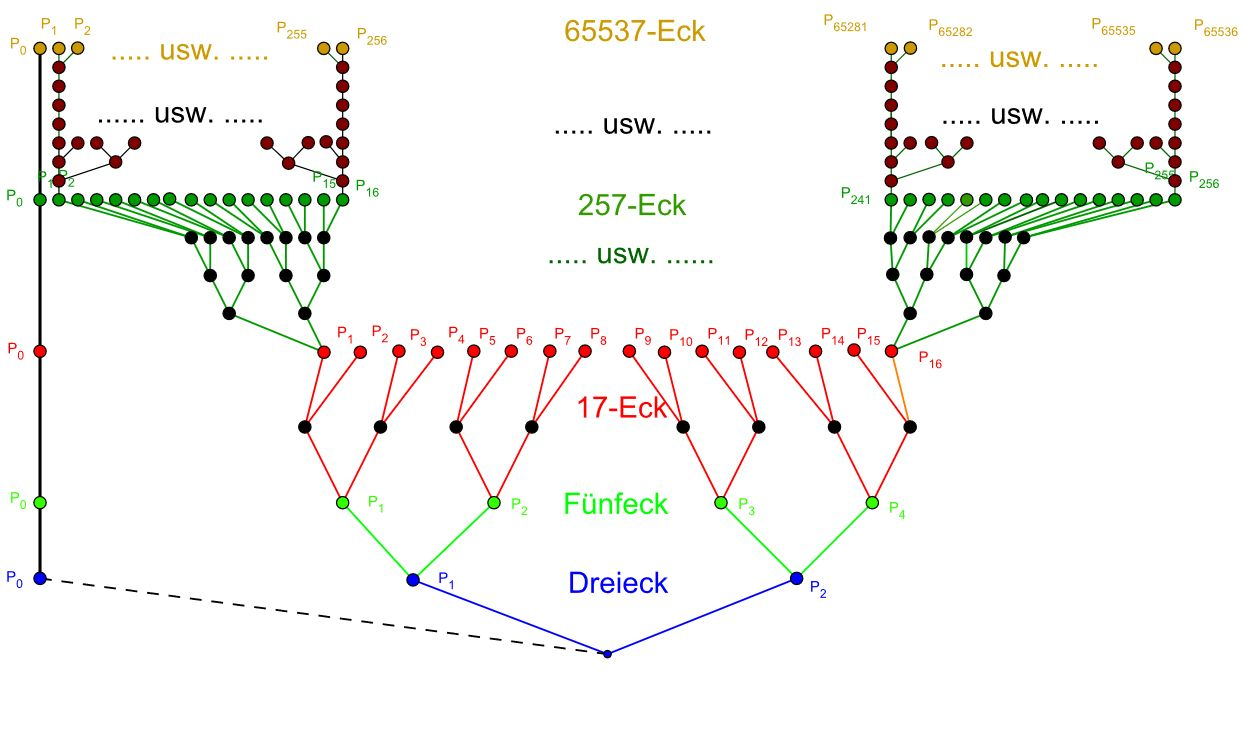
\includegraphics[width=.7\textwidth]{Baum.jpg}
\end{center}

\paragraph{Reguläres 17-Eck:}
Die praktische Umsetzung der Konstruktion des regulären 17-Ecks und des
regulären 257-Ecks wurde von \textsc{Gauss} nicht erbracht, sondern für das
reguläre 17-Eck erstmalig 1825 von
\textsc{Erchinger}\footnote{\url{http://de.wikipedia.org/wiki/Siebzehneck}
  (abgerufen am 01.09.2011).}. Für eine illustrierte Konstruktionsbeschreibung
des regulären 17-Ecks als pdf-Datei siehe \texttt{17Eck.pdf}.

\paragraph{Reguläres 257-Eck:}
Die erste Konstruktion des regulären
257-Ecks\footnote{\url{http://de.wikipedia.org/wiki/257-Eck} (abgerufen am
  03.06.2016).} beschrieb 1819, gedruckt 1822, \textsc{Paucker} (1787-1855)
\cite{Paucker1822}, später 1832 \textsc{Richelot} (1808-1875)
\cite{Richelot1832}. Für die Konstruktion des regulären 257-Ecks folgten
später weitere Arbeiten (\textsc{deTemple} 1991 \cite{deTemple1991},
\textsc{Gottlieb} 1999 \cite{Gottlieb1999}), die u.a. das Ziel hatten, die
Anzahl der zur Konstruktion nötigen Kreise und Geraden zu reduzieren.
\textsc{Paucker} zitiert aus einem Brief von \textsc{Gauss} an ihn von 1820,
worin \textsc{Gauss} auf eigene Überlegungen und Rechnungen zum regulären
257-Eck im Jahre 1796 hinweist. \textsc{Paucker} vergleicht seine Ausdrücke
mit denen von \textsc{Gauss} und bemerkt strukturelle Übereinstimmung in den
Gleichungen, nur die Bezeichnungen waren unterschiedlich. Das sollte bedeuten,
dass bereits \textsc{Gauss} einen gleichen oder vergleichbaten Ansatz zur
Herleitung verwendet hatte. \textsc{Gauss} verweist explizit auf die
Verwendung der Primitivwurzel 3 ([8], S. 217-219). \textsc{Paucker} benutzt
als erster auch die Schreibweise mit den indizierten Buchstaben $A, B, ...,
G$, wie sie auch hier in der Herleitung verwendet wird.

Zur analytischen Herleitung siehe unten.

Eine Vorstellung von der Konstruktion des regulären 257-Ecks (4) im
Internetzeitalter liefert ein Video (mp4-Format -- etwa 40 MByte, avi-Format
-- etwa 400 MByte; Quelle zu ergänzen). Mit Hilfe des modernen interaktiven
Geometrieprogramms \emph{Geogebra} wurde die Konstruktion vom Autor auf der
Grundlage einer
Internetquelle\footnote{\url{http://it.wikipedia.org/wiki/257-gono} (abgerufen
  am 01.09.2011).} und damit \cite{deTemple1991} durchgeführt. Zur Lösung der
vielfach zu lösenden quadratischen Gleichungen wurde ein auch für die
Schulmathematik interessanter Ansatz verwendet: Die Kreise von
\textsc{Carlyle}\footnote{\url{http://it.wikipedia.org/wiki/Cerchio_di_Carlyle}
  (abgerufen am 01.09.2011).} (1795-1881). Das Prinzip ist aus der Abbildung
zu erkennen.

\begin{center}
  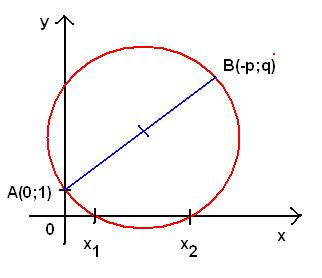
\includegraphics[width=.7\textwidth]{CarlyleKreis.jpg}
\end{center}

Mit einigen Hilfsschritten benötigt man für die Konstruktion der Seitenlänge
rund 380 Schritte, für das komplette 257-Eck etwa 1170 Schritte. Die
Konstruktion der Mittelsenkrechten einer Strecke wird dabei häufig benötigt.
Diese ist als \emph{Werkzeug}, gewissermaßen als Macro, vordefiniert, und
lässt sich sehr bequem in \emph{Geogebra} nutzen. Bei ausschließlicher
Verwendung von Kreisen und Geraden ist die Anzahl der Konstruktionsschritte
deutlich größer. \emph{Geogebra} arbeitet intern mit gerundeten Dezimalzahlen,
also nicht mit symbolischen Ausdrücken. Die Anzahl der Dezimalstellen kann man
wählen. Im Video (Quelle zu ergänzen) sieht man bei einen Blick in das
Algebrafenster, mit welch hoher numerischen Stabilität (vom Autor 12
Nachkommastellen gewählt) das Programm für jede der 257 gleich langen Seiten
gleiche Werte (0.02444758303) ausrechnet.

Zwei kleine Hinweise dazu:
\begin{itemize}[noitemsep]
\item Unter Verwendung der minimalen Schrittzeit von 1 s bei der Darstellung
  einer Konstruktion in Geogebra dauert die Konstruktion auch etwa 1170 s,
  also etwa 20 min. Der mögliche Schnelldurchlauf des Videos gestattet eine
  deutliche Verringerung dieser Zeit.
\item Dem Betrachter wird durch das Video auch die Auswahl einer geeigneten
  Vergrößerung abgenommen, um die während der Konstruktion relevanten Objekte
  gut sichtbar werden zu lassen.
\end{itemize}

\subsection*{Analytische Herleitung der Konstruktion des regulären 257-Ecks}

Die moderne Begründung der Konstruierbarkeit des regulären 257-Ecks mit Zirkel
und Lineal erfolgt durch Folgerungen aus der \textsc{Galois}-Theorie. Der
geneigte Leser sei auf einschlägige Arbeiten verwiesen, u. a. in
Kurzform\footnote{\url{http://de.wikipedia.org/wiki/Konstruierbare_Polygone}
  (abgerufen am 20.05.2016)}, ausführlicher \cite{Bishop1978} mit Anmerkungen
zur Konstruktion des regulären 257-Ecks.

Die Konstruktion soll mit einfacheren Mittel begründet und nachvollziehbar
hergeleitet werden. Wesentliche Stütze ist die Arbeit \cite{deTemple1991}.

Der Mittelpunkt des 257-Ecks liegt im Ursprung eines komplexen
Koordinatensystems, d.h. die reellen Zahlen finden sich auf der Abszissenachse
und die Vielfachen von $\ii$ mit $\ii^{2}=-1$ auf der Ordinatenachse.

Alle Eckpunkte des 257-Ecks liegen auf einen Kreis. Zur Vereinfachung wählt
man den Einheitskreis mit dem Radius $r = 1$. Das 257-Eck wird so gedreht,
dass ein Eckpunkt der Punkt $(0,1)$ ist. Die Eckpunkte des 257-Ecks erfüllen
die komplexe Gleichung $z^{257} = 1$.

Die Gleichung $z^{257} =1$ soll im Bereich der komplexen Zahlen gelöst werden,
also $z^{257} - 1 = 0$. Der Winkel $\alpha$ mit dem Scheitelpunkt im Ursprung
des Koordinatensystems zwischen Abszissenachse und Strahl durch den Punkt
$P_1$, beträgt in Bogenmaß $\alpha= \frac{2\pi}{257}$. Also ist $z =
\cos(\alpha) + \ii\sin(\alpha)$.

So ist nach der \textsc{Euler}schen Identität $z =
\mathrm{e}^{\frac{2\pi\ii}{257}}$.  Es ist überhaupt nicht schwierig, wenn man
es mit komplexen Zahlen zu tun hat. Man kann über den Realteil von $z$, also
$\cos(\alpha)$, der auf der Abszissenachse zu finden ist, den Schnittpunkt mit
dem Einheitskreis finden. Dieser Punkt ist dann einer der Eckpunkte des
regulären 257-Ecks.

Im Bereich der komplexen Zahlen hat die Gleichung $z^{257} = 1$ nach dem
\textsc{Gauss}schen Fundamentalsatz der Algebra 257 Lösungen. Wie man sofort
sieht, ist $z = 1$ eine (triviale) reelle Lösung. Die anderen 256 Lösungen
ergeben sich als Nullstellen des Polynoms
\begin{gather*}
   \frac{z^{257}-1}{z-1}=z^{256}+z^{255}+\ldots+z^3+z^2+z+1.\tag{2}
\end{gather*}
Diese Nullstellen $z_i$, $i=0,\ldots,256$, lassen sich alle als $z_i=\zeta^i$
für eine geeignete komplexe Zahl $\zeta$ darstellen; die Multiplikation zweier
Nullstellen $z_i\cdot z_j=\zeta^{i+j}$ entspricht dabei der Addition der
Exponenten, wobei wegen $\zeta^{257}=1$ der Exponent $i+j$ modulo 257
reduziert, also in der additiven Gruppe des Restklassenrings $\Z_{257}$
gerechnet werden kann.

Die Nullstellen $z_i\neq 1$ entsprechen dabei den primitiven Restklassen
$\Z_{257}^\ast$, die ihrerseits eine endliche multiplikative Gruppe bilden.
Diese Gruppe kann zyklisch erzeugt werden, d.h. es gibt ein Element $g\in
\Z_{257}^\ast$, so dass
\begin{gather*}
  \Z_{257}^\ast=\cbr{1,g,g^2,g^3,\ldots,g^{256}}\quad \text{und}\quad g^{257}=1
\end{gather*}
gilt.  Damit lassen sich die Nullstellen des Polynoms (2) als 
\begin{gather*}
  \zeta = \zeta^{g^0}, \zeta^{g^1}, \zeta^{g^2}, \zeta^{g^3}, \ldots,
  \zeta^{g^{256}}
\end{gather*}
darstellen, wobei $\zeta^{g^{257}} = \zeta^1$ gilt.  Eine solche Zahl $g$
heißt \emph{Primitivwurzel modulo 257}. Für alle (bekannten)
\textsc{Fermat}schen Primzahlen größer als 3 ist $g=3$ eine solche
Primitivwurzel. 

Bei endlichen Mengen versteht man unter der Mächtigkeit einer Menge $M$ die
Anzahl der Elemente von $M$. Aus der Rechnung mit Restklassen lässt sich
offensichtlich problemlos der folgende Satz ableiten:
\begin{quote}
  \textbf{Satz:} Es sei $i$ die Mächtigkeit der Menge $M_n$ der Restklassen
  $\pmod{n}$, $j$ die Mächtigkeit der Menge $M_{2n}$ der Restklassen
  $\pmod{2n}$, so ist $j = 2 \cdot i$ und $M_n \subset M_{2n}$.
\end{quote}
Zur Veranschaulichung: Ein Zifferblatt einer Analoguhr ist häufig in 12
gleiche große Winkel eingeteilt. Wir geben nicht die Gesamtzahl der Stunden
seit irgendeinem Starttermin an, sondern die Restklasse mod 12. Diese ist auf
dem Zifferblatt ablesbar, z. B. als Punkt oder Strecke auf dem Schenkel des
entsprechenden Winkels. Nun soll die Angabe verfeinert werden: Jede Stunde
soll in Halbstunden eingeteilt werden. Es kommen also zusätzlich zu den
bestehenden 12 Restklassen noch 12 neue Restklassen hinzu. Die Anzahl der
Restklassen verdoppelt sich. Die ehemaligen 12 Restklassen gibt es auch bei
der neuen Einteilung noch.

Wie findet man eine nichttriviale Lösung der Gleichung (2)?  Ein möglicher
Ansatz ist die Zerlegung der Menge der 256 Lösungen in zwei gleichmächtige
Mengen $M_0$ und $M_1$. Es sollen daraus zwei reelle Zahlen $A_0$ und $A_1$
konstruiert werden. Aus ihnen kann mit Hilfe des \textsc{Vieta}schen
Wurzelsatzes (\textsc{Vieta} 1540-1603) eine quadratische Gleichung bestimmt
werden.

Kriterium der Auswahl ist der Index der $z_i$ ($i = 1, 2, ..., 257$). Man
verwendet die Restklassen der Indizes modulo 2, also 0 oder 1. (Die Restklasse
kommt in den Indizes der Mengen $M_0$ und $M_1$ zum Ausdruck). So nehmen wir
alle 128 Lösungen $z_i = z^{i \pmod{257}}$ mit geraden Indizes in die Menge
$M_0$, die restlichen 128 Lösungen in die andere Menge $M_1$. Es sei 
\begin{align*}
  A_0&= \sum_{0<i<256, i\ \text{ungerade}}{z^{3^i \pmod{257}}}
  =z^3+z^{27}+\ldots+z^{238}+z^{86} \quad \text{und}\\
  A_1 &= \sum_{0\le i <256, i\ \text{gerade}}{z^{3^i \pmod{257}}} =
  z^1+z^9+\ldots+z^{165}+z^{200}.
\end{align*}
% Maxima:
%% tellrat((z^(257)-1)/(z-1));
%% algebraic:true;
%% A0:sum(z^(power_mod(3,(2*i+1),257)),i,0,127);
%% A1:sum(z^(power_mod(3,(2*i),257)),i,0,127);
%% ratsimp(A0+A1);  /*  - 1 */
%% ratsimp(A0*A1);  /* - 64 */

Wie man sofort sieht, ist $A_0 + A_1 = -1$. Das Produkt $A_0 \cdot A_1$ ergibt
nach Ausmultiplizieren eine Summe von $128 \cdot 128 = 16384$ Summanden, die
sich zu $-64$ vereinfachen lässt. Beides kann mit \textsc{Maxima}\footnote{Ein
  freies CAS, das von Lehrern gern eingesetzt wird,
  \url{http://maxima.sourceforge.net/}} schnell nachgeprüft werden:
\begin{code}
tellrat((z\pw(257)-1)/(z-1));\\
algebraic:true;\\
A0:sum(z\pw(power\_mod(3,(2*i+1),257)),i,0,127);\\
A1:sum(z\pw(power\_mod(3,(2*i),257)),i,0,127);\\
ratsimp(A0+A1); /*  -1 */\\
ratsimp(A0*A1); /* -64 */
\end{code}

Die Gleichungen $A_0 + A_1 = -1$ und $A_0 \cdot A_1 = -64$ führen nach dem
\textsc{Vieta}schen Wurzelsatz zu der quadratischen Gleichung $s^2 + s - 64 =
0$ mit 
\begin{gather*}
  A_0=\frac{-1+\sqrt{257}}{2}\quad\text{und}\quad A_1=\frac{-1-\sqrt{257}}{2}.
\end{gather*}
$A_0$ und $A_1$ sind beides reelle Zahlen. Man findet sie auf der
Abzissenachse des komplexen Koordinatensystems (siehe Schritt 36 der
Konstruktion des regulären 257-Ecks).

Als nächstes zerlegt man die Menge der Lösungen mit geraden Indices $M_{0}$
weiter in zwei gleichmächtige Mengen $M_{0,0}$ und $M_{0,2}$. In der Menge
$M_{0,0}$ sind jetzt alle Lösungen mit durch 4 teilbaren Indizes und in der
Menge $M_{0,2}$ alle Lösungen mit geradem, aber nicht durch 4 teilbaren
Indizes.  Man wählt den Ansatz 
\begin{align*}
  B_0 &= z^1 + z^{81} + z^{136} + ... + z^{240} + z^{165}\quad\text{und}\\ B_2
  &= z^9 + z^{215} + z^{196} + ... + z^{104} + z^{200}.
\end{align*}
Es ist $B_0 + B_2 = A_0$ und $B_0 \cdot B_2 = -164$. In den Tabellen 3 und 4
ist diese Multiplikation vollständig dargestellt.

\textsc{Maxima} liefert allerdings ein anderes Ergebnis (Fortsetzung der
Rechnung oben): 
\begin{code}
B0:sum(z\pw(power\_mod(3,(4*i),257)),i,0,63);\\
B2:sum(z\pw(power\_mod(3,(4*i+2),257)),i,0,63);\\
ratsimp(B0+B2+A0); /*  - 1 */\\
ratsimp(B0*B2);  /* - 16 */
\end{code}

% Maxima: Fortsetzung
%% B0:sum(z^(power_mod(3,(4*i),257)),i,0,63);
%% B2:sum(z^(power_mod(3,(4*i+2),257)),i,0,63);
%% ratsimp(B0+B2+A0); /*  - 1 */
%% ratsimp(B0*B2);  /* - 16 */

Daraus erhält man die quadratische Gleichung $s^{2}- A_{0} \cdot s - 16 = 0$
mit den Lösungen
\begin{gather*}
  B_0 = \frac{A_0}{2}+ \sqrt{\br{\frac{A_0}{2}}^2+16}\quad\text{und}\quad B_2
  = \frac{A_0}{2}- \sqrt{\br{\frac{A_0}{2}}^2+16}.
\end{gather*}

\newpage


\begin{thebibliography}{xxx}
\bibitem{GaussTagebuch} Mathematisches Tagebuch 1796-1814 von Carl Friedrich
  Gauss. Mit einer historischen Einführung von Kurt-R. Biermann. Ostwalds
  Klassiker der exakten Wissenschaften, Band 256. Leipzig 1976.
\bibitem{Patzschke2002} Patzschke, Jürgen: Carl Friedrich Gauss und das
  Siebzehneck -- Teil I. In \emph{Wurzel}, Heft 5, 2002, S. 15-24.
\bibitem{Paucker1822} Paucker, Georg: Geometrische Verzeichnung des
  regelmässigen Siebzehn-Ecks und Zweyhundertsiebenundfunfzig-Ecks in den
  Kreis. In \emph{Jahresverhandlungen der kurländischen Gesellschaft für
    Literatur und Kunst}, Zweyter Band, Mitau 1822, S. 160-219.
\bibitem{Richelot1832} Richelot, Friedrich Julius: De resolutione algebraica
  aequationis $x^{257} = 1$, sive de divisione circuli per bisectionem anguli
  septies repetitam in partes 257 inter se aequales commentatio coronata. In
  \emph{Journal für die reine und angewandte Mathematik}, Nr. 9, 1832,
  S. 1-26, 146-161, 209-230 und 337-358.
\bibitem{deTemple1991} DeTemple, Duane W.: Carlyle Circles and the Lemoine
  Simplicity of Polygonal Constructions. In \emph{Amer. Math.  Monthly},
  vol. 98, 1991, S. 97-108.
\bibitem{Gottlieb1999} Gottlieb, Christian: The Simple and Straightforward
  Construction of the Regular 257-gon. In \emph{Mathematical Intelligencer},
  vol. 21, No. 1, 1999, S. 31-37.
\bibitem{Bishop1978} Bishop, Wayne: How to construct a regular polygon. In
  \emph{Amer. Math. Monthly}, vol. 85, 1978, S. 186-188.
\bibitem{Polster2016} Polster, Steffen: Software \emph{Mathematik Alpha 2016},
  \url{http://mathematikalpha.de}.
\bibitem{Hermes1898} [17] Hermes, Johann Gustav: Diarium zur Kreisteilung,
  Königsberg 1879, (1879 begonnen - d. A.)
\bibitem{Hermes1894} [18] Hermes, Johann Gustav: Ueber die Teilung des Kreises
  in 65537 gleiche Teile. In \emph{Nachrichten von der Gesellschaft der
  Wissenschaften zu Göttingen}, Mathematisch-Physikalische Klasse. Göttingen,
  1894, S. 170–186.
%[19] http://facstaff.susqu.edu/brakke/constructions/65537-gon.m.txt (abgerufen am 06.06.2017)
\end{thebibliography}

\end{document}

Die restlichen Lösungen aus der Menge M_0 sind diejenigen mit ungeraden
Indices. Sie werden in zwei gleichmächtige Mengen M_{0; 1} und M_{0; 3}
aufgeteilt. In M_{0; 1} sind jetzt alle Lösungen, deren Indices bei Division
durch 4 den Rest 1 lassen, und in M_{0; 3} alle anderen noch nicht in M_{0;
  0}, M_{0; 1} und M_{0; 2} enthaltenen Lösungen, also alle deren Indices bei
Division durch 4 den Rest 3 lassen. Wir wählen B_1 = z^3 + z^{243} + z^{151} +
... + z^{206} + z^{238} und B_3 = z^{273} + z^{131} + z^{74} + ... + z^{55} +
z^{86}. Es ist B_1 + B_3 = A_1 und B_1 \cdot B_3 = -16. Man erhält daraus die
quadratische Gleichung s^2 - A_1 \cdot s - 16 = 0, deren Lösungen B_1 =
\frac{A_1}{2}+ \sqrt{\left({\frac{A_1}{2}}\right)^2+16} und B_3 =
\frac{A_1}{2}- \sqrt{\left({\frac{A_1}{2}}\right)^2+16} sind.

Zur Illustration wird auf die Tabellen 5 und 6 verwiesen.

Die Einteilung der Indices in die Mengen M_0 bis M_{0; 3} erfolgte nach ihren
Restklassen mod 2 und dann mod 4. (Es entstanden die Werte A_i\: (i = 0;
1),\:\: B_j\: (j = 0; 1; 2; 3).


Dieses Prinzip soll weiter verfolgt werden. Es werden im Folgenden mit
geeigneten Restklassen mod 8, mod 16, mod 32, mod 64 und mod 128
ausgewählt. Dann entstehen die Werte C_k\: (k = 0; 1; ...; 7), \:\: D_m\: (m =
0; 1; ...; 15),\:\: E_n\: (n = 0; 1, ...; 31),:\: F_o\: (o = 0; 1; ...; 63)
und G_p\: (p = 0; 1; ...; 127). (Die Bezeichnung der Restklassen mit diesen
Buchstaben A, B, ..., G mit den jeweiligen Indices erfolgt in gleicher Weise
wie die Bezeichnung von Punkten, die während der Konstruktion des 257-Ecks
entstehen.)

Bei jeder Einteilung der Indices in Teilmengen wird immer die gleiche Anzahl
in Klassen aufgeteilt. Aus diesem Grund gilt: \sum_{i=0}^{1}A_i =
\sum_{j=0}^{3}B_j =\sum_{k=0}^{7}C_k =\sum_{m=0}^{15}D_m =\sum_{n=0}^{31}E_n
=\sum_{o=0}^{63}F_o =\sum_{p=0}^{127}G_p =1 Wie bereits erwähnt, bilden die
Restklassen mod p, also auch mod 257, eine multiplikative Gruppe. Bei der
Multiplikation von Potenzen mit gleicher Basis wird die Basis beibehalten und
die Exponenten addiert. Es reicht also aus, wenn man die Addition der
Exponenten betrachtet. Solch eine Additionstafel ist in Tabelle 7 vollständig
dargestellt. (In der Kopfzeile bzw. -spalte sind die Elemente der Menge M_{0}
für den Fall der Restklassen 0 und 4 mod 8 angegeben.)


Nach (**) gilt C_0 + C_4 = B_0. Um mit dem Wurzelsatz von \textsc{Vieta} eine
quadratische Gleichung erhalten zu können, benötigt man noch einen
äquivalenten Term für C_0 \cdot C_4. Dieser soll als Linearkombination aus den
bekannten B_j\: (j = 0; 1; 2; 3) und A_i\: (i = 0; 1) gebildet werden. So ist
also

C_0 \cdot C_4 = n_{B_0} \cdot B_0 + n_{B_1} \cdot B_1 + n_{B_2} \cdot B_2 +
n_{B_3} \cdot B_3 + n_{A_0} \cdot A_0 + n_{A_1} \cdot A_1 + n_0 ,

wobei die Koeffizienten n_q\in\mathbb{Z} sein sollen. Ganze Zahlen sind mit
Zirkel und Lineal sehr leicht zu konstruieren. Man erhält somit eine
inhomogene lineare diophantische Gleichung. Zu deren Lösung gibt es
Algorithmen. Hier wird modulo 257 gerechnet, was deren Anwendung etwas
erschwert. Zum Glück ist es aber im vorliegenden Fall leicht die Lösung der
vorliegenden diophantischen Gleichung auch ohne großen Rechenaufwand zu
finden.

In Tabelle 8 wird angegeben, wie oft die einzelnen Restklassen auftreten. Man
erkennt, es gibt genau drei Fälle: 2, 4 und 5. Subtrahiert man von jeder
Anzahl 2, so erhält man 0, 2 und 3. Für Restklasse 1 mod 2 (rot markiert)
ergibt sich jeweils als Anzahl 3, und für Restklasse 2 mod 4 (blau markiert)
jeweils die Anzahl 2. Daraus ergibt sich:

C_0 \cdot C_4 = 3 \cdot \color {red} {A_1} + 2 \cdot \color {blue} {B_2} - 2. Analog erhält man:
C_1 \cdot C_5 = 3 \cdot A_0 + 2 \cdot B_3 - 2,
C_2 \cdot C_6 = 3 \cdot A_1 + 2 \cdot B_0 - 2,
C_3 \cdot C_7 = 3 \cdot A_0 + 2 \cdot B_1 - 2
. Es gilt C_0 + C_4 = B_0. Das erklärt sich sofort aus (**). So ergeben sich
auch

C_1 + C_5 = B_1, C_2 + C_6 = B_2 und C_3 + C_7 = B_3.
Eine der nach dem Satz von \textsc{Vieta} zu bildenden 4 quadratischen Gleichungen
lautet dann z.B. s^2 - B_0 \cdot s + 3 \cdot A_1 + 2 \cdot B_2 - 2 = 0.


Völlig analog werden als nächstens geeignete Restklassen mod 16 ausgewählt und
Linearkombinationen gebildet. Wir erhalten:

D_0 \cdot D_{ 8} = A_0 + C_0 + C_2 + 2 \cdot C_5,
D_1 \cdot D_{ 9} = A_1 + C_1 + C_3 + 2 \cdot C_6,
D_2 \cdot D_{10} = A_0 + C_2 + C_4 + 2 \cdot C_7,
D_3 \cdot D_{11} = A_1 + C_3 + C_5 + 2 \cdot C_0,
D_4 \cdot D_{12} = A_0 + C_4 + C_6 + 2 \cdot C_1,
D_5 \cdot D_{13} = A_1 + C_5 + C_7 + 2 \cdot C_2,
D_6 \cdot D_{14} = A_0 + C_6 + C_0 + 2 \cdot C_3,
D_7 \cdot D_{15} = A_1 + C_7 + C_1 + 2 \cdot C_4.
Es gilt: D_0 + D_8 = C_0, D_1 + D_9 = C_1 usw.
Es werden 8 quadratische Gleichungen gebildet, u. a. s^2 - C_0 \cdot s + A_0 +
C_0 + C_2 + 2 \cdot C_5 = 0.


Jetzt wird das Verfahren mit Restklassen mod 32 fortgesetzt. Man erhält:
E_{ 0} \cdot E_{16} = D_{ 0} + D_{ 1} + D_{ 2} + D_{ 5},
E_{ 1} \cdot E_{17} = D_{ 1} + D_{ 2} + D_{ 3} + D_{ 6},
E_{ 7} \cdot E_{23} = D_{ 7} + D_{ 8} + D_{ 9} + D_{12},
E_{ 8} \cdot E_{24} = D_{ 8} + D_{ 9} + D_{10} + D_{13},
E_{ 9} \cdot E_{25} = D_{ 9} + D_{10} + D_{11} + D_{14},
E_{31} \cdot E_{15} = D_{15} + D_{ 0} + D_{ 1} + D_{ 4}.
Es ist E_{ 0} + E_{16} = D_{ 0} usw. Diesmal werden 6 quadratische Gleichungen
gebildet, u. a. s^2 - D_0 \cdot s + D_{ 0} + D_{ 1} + D_{ 2} + D_{ 5}.

Aus den anderen Restklassen mod 32 können weitere 10 Gleichungen gebildet
werden. Sie sind aber für den Fortgang der Herleitung entbehrlich. Sie werden
nur zum Zwecke der Vollständigkeit hier aufgeführt: {\scriptsize E_{ 2} \cdot
  E_{18} = D_{ 2} + D_{ 3} + D_{ 4} + D_{ 7},\: E_{ 3} \cdot E_{19} = D_{ 3} +
  D_{ 4} + D_{ 5} + D_{ 8},\: E_{ 4} \cdot E_{20} = D_{ 4} + D_{ 5} + D_{ 6} +
  D_{ 9},\: E_{ 5} \cdot E_{21} = D_{ 5} + D_{ 6} + D_{ 7} + D_{10},\: E_{ 6}
  \cdot E_{22} = D_{ 6} + D_{ 7} + D_{ 8} + D_{11}}

{\scriptsize E_{10} \cdot E_{26} = D_{10} + D_{11} + D_{12} + D_{15},\: E_{11}
  \cdot E_{27} = D_{11} + D_{12} + D_{13} + D_{ 0},\: E_{12} \cdot E_{28} =
  D_{12} + D_{13} + D_{14} + D_{ 1},\: E_{13} \cdot E_{29} = D_{13} + D_{14} +
  D_{15} + D_{ 2},\: E_{14} \cdot E_{30} = D_{14} + D_{15} + D_{ 0} + D_{ 3}}.


Als nächstens betrachten wir Restklassen mod 64. Aus der Additionstafel (siehe
Tabelle 9) ergibt sich zunächst:


F_0 \cdot F_{32} = \color {red} {F_{33}} + \color {green} {F_{55}} + \color
{blue} {F_{23}} + \color {gray} {F_1}

Offensichtlich ist x mod 32 = (x + 32) mod 32. Daraus ergibt sich:F_{ 0} \cdot
F_{32} = E_{ 1} + E_{23}.

Analog: F_{24} \cdot F_{56} = E_{15} + E_{25}.

Es ist F_{ 0} + F_{32} = E_{ 0} und F_{24} + F_{56} = E_{24}.
Hier sind zwei quadratische Gleichungen zu bilden, um F_{24}, F_{56}, F_{ 0}
und F_{32} zu finden, also

s^2 - E_{ 0} \cdot s + E_{ 1} + E_{23} = 0, s^2 -
E_{24} \cdot s + E_{15} + F_{25} = 0

Nun noch mod 128: G_{ 0} \cdot G_{64} = F_{56}, G_{ 0} + G_{64} = F_{ 0}.
Daraus erhält man mit Hilfe von s^2 - F_{ 0} \cdot s + F_{56} = 0
u. a. G_{64}.


Es wurde jener Wert für z gefunden, dessen Exponent beim Potenzieren von 3 mod
257 den Rest 64 ergibt. Nach Tabelle 1 ist ein 32 ein solcher Wert. Das heißt
z=\textrm{e}^{\left(\frac{2\pi \textrm{i}}{257}\right)^{32}}=
\textrm{e}^{\left(\frac{2\pi \textrm{i} \cdot 32}{257}\right)}
=\textrm{e}^{\left(32\cdot\frac{2\pi \textrm{i}}{257}\right)} und damit der
Realteil \cos\left(32\cdot\alpha\right). Auf den ersten Blick führt aber
G_{64} \approx 1.8 zu einem Widerspruch. G_{64} gibt geometrisch gesehen die
Sehnenlänge zwischen zwei Eckpunkten P_{\:i} und P_{\:i+32} (i = 0; \ldots;
256) des 257-Ecks an. Das bedeutet: G_{64}/2 ist die halbe Sehnenlänge, ist
auch eine Lösung der Gleichung x^{256} - 1 = 0 und entspricht damit \cos
\left({16\alpha}\right). G_{64}/2 ist die Abszisse des Eckpunktes P_{17} des
regulären 257-Ecks. Mit der fortwährenden Abtragung der Sehnenlänge
\overline{P_{\:1}P_{17}} (mit dem Zirkel) erhält man alle weiteren Eckpunkte
des regulären 257-Ecks: In der beigefügten Konstruktion des regulären 257-Eck
Schritt 398 bis 911.


Reguläres 65537-Eck:

Die Umsetzung der Konstruierbarkeit des regulären 65537-Ecks hatte sich HERMES
(1846-1912) vorgenommen. Er legte die Arbeit [17] 1894 vor. Grundlage war
[18]. Obwohl in der Arbeit das 65537-Eck nicht konstruiert wird, gibt sie
einen genauen Überblick, wie man es machen könnte. Felix KLEIN schlug vor,
diese Arbeit als Dissertation anzuerkennen. Bekanntermaßen wird sie heute in
einem speziellen mit Stoff ausgeschlagenen Holzkoffer im Mathematischen
Institut der Georg-August-Universität in Göttingen aufbewahrt. Der Koffer ist
Teil der Modellsammlung des Mathematischen Instituts der Universität
Göttingen.

Der Autor bekam anlässlich der Bundesrunde der 49. Mathematik-Olympiade 2010
in Göttingen die besondere Gelegenheit geboten, die besagte Arbeit persönlich
in Augenschein nehmen und darin lesen zu dürfen. Auch durften Fotos
angefertigt werden.

Die Arbeit umfasst 221 Seiten, die in einer der Deutschen Kurrentschrift
ähnlichen Schrift geschrieben sind. Die Seiten haben z. T. unterschiedliches
Format. Einige davon mussten zusammengeklappt werden, um ein aus heutiger
Sicht unstandardisiertes Format, dass zwischen A4- und A3-Größe liegt, zu
erhalten. Einige Seiten sind aus mehreren Stücken zusammengeklebt worden
bzw. es sind Korrekturen eingearbeitet worden. Möglicherweise hätte eine
Abschrift der betreffenden Seiten einen zu hohen Zeitaufwand bedeutet, der den
Anfertigungszeitraum der Arbeit noch weiter ausgedehnt hätte. Wenn man die
Seiten betrachtet, gewinnt man einen Eindruck vom außerordentlichen Fleiß und
der Ausdauer von HERMES, der ab 1879 mehr als 10 Jahre daran arbeitete. Leider
können die angefügten Bilder nur einen unzureichenden Eindruck davon
vermitteln. In der Arbeit werden sehr systematisch Betrachtungen zu Lösungen
der entsprechenden Kreisteilungsgleichungen gemacht, die zur Konstruktion des
regulären 5-, 17-, 257- und 65537-Eck führen. Schon im benötigten Platz für
seine Betrachtungen zu diesen Polygonen wird der immens steigende Rechen- und
Schreibaufwand deutlich, um die Lösungen der Kreisteilungsgleichungen zu
finden. Dazu hat er eigene Symbole entwickelt, um die Übersichtlichkeit und
Kompaktheit der Darstellung zu erhöhen. HERMES macht in seiner Arbeit
deutlich, dass er nach Analogien, Perioden und ähnlichem in den Lösungen der
Kreisteilungsgleichung für das reguläre 65537-Eck gesucht hat5 .


Im Folgenden werden einige Bemerkungen bei der Herleitung der Konstruktion des
regulären 65537-Ecks gemacht, die auch die immense Arbeitsleistung von HERMES
noch mehr verdeutlichen.

BRAKKE hat mit einem sehr ähnlichen Ansatz, wie oben im Text beim regulären
17-Eck und 257-Eck beschrieben, verschachtelte quadratische Gleichungen mit
Computerunterstützung hergeleitet und als Mathematica-File veröffentlicht
[19]. Damit lässt sich in kurzer Zeit die Abszisse des 8192. Eckpunktes des
regulären 65537-Ecks berechnen.

Der Autor hat die Gleichungen so umgeformt und umkodiert, dass die von ihm oben benutzte Notation der Restklassen verwendet werden kann. So lässt sich das reguläre 65537-Eck, wieder ähnlich wie das reguläre 257-Eck, konstruieren.
Die Anzahl der ineinander verschachtelten quadratischen Gleichungen verdoppelt
sich mit jeder Erhöhung der "Verteilebene" A, B, C, ... ,R6. Ein Eckpunkt ist
wieder mit dem Punkt (1;0) frei gewählt.

Da aber die Herleitung der Abszisse eines weiteren Eckpunktes, hier des
8192. Eckpunktes7 , letztlich ausreicht um daraus das gesamte reguläre
65537-Eck zu konstruieren, muss man nicht alle quadratischen Gleichungen
lösen. Ab der Verteilebene K benötigt man immer weniger Gleichungen (siehe
nachstehende Tabelle 10). Die Gesamtanzahl der benutzten quadratischen
Gleichungen beträgt 1141. (Zum Vergleich: Beim regulären 257-Eck waren es
"nur" 24.) Nicht immer benötigt man beide Lösungen für die weitere
Rechnung. Die nicht weiter verwendeten Lösungen werden in der Tabelle
durchgekreuzt. Die komplette Darstellung aller Gleichungen würde sehr viel
Platz beanspruchen. Aus diesem Grund können die Gleichungen in einer pdf-Datei
( Verschachelte quadratische Gleichungen zur Berechnung von cos(2pi/65537))
betrachtet werden. In Tabelle 10 sind einige Beispiele angegeben.

Ausgangspunkt der Überlegungen ist wieder der beim regulären 17- und 257-Eck
erfolgreich genutzte Ansatz die Restklassen (außer der Restklasse 0), jetzt
mod 65537, in zwei gleichmächtige Mengen A0 und A1 aufzuteilen. Der weitere
Weg ist ebenfalls oben ausführlich beschrieben. Beim regulären 257-Eck wurde
die Bildung der Linearkombinationen aus den Restklassen anschaulich mit den
Multiplikationstafeln beschrieben. Ein viel effektiverer Weg, vor allem mit
Computerhilfe, für die Ermittlung jeder der Linearkombinationen ist, lineare
Gleichungssysteme aufzustellen und dann zu lösen.

Deutlich wird, dass man die quadratischen Gleichungen in einer bestimmten
Verteilebene nur mit den Lösungen der quadratischen Gleichungen voriger
Verteilebenen aufstellen kann. In den Linearkombinationen sind Lösungen
quadratischer Gleichungen von bis zu 7 vorhergehender Verteilebenen
enthalten. Für die Aufstellung der quadratischen Gleichungen kommt der Satz
von \textsc{Vieta} zur Anwendung.

Verteilebene 	mod n 	Anzahl der quadratischen Gleichungen 	davon
verwendet für weitere Rechnungen 	Beispiel

A 	2 	1 	1 	A0 + A1 = -1
A0 ∙ A1 = -16384

quadratische Gleichung: s2 + 1 ∙ s - 16384 = 0
B 	4 	2 	2 	B0 + B2 = A0
B0 ∙ B2 = - 4096
allgemein: Bi ∙ Bi+2= -4096 (i= 0, 1)

quadratische Gleichung: s2 - A0 ∙ s - 4096 = 0
C 	8 	4 	4 	C0 + C4 = B0
C0 ∙ C4 = - 16 ∙ A0 - 32 ∙ B0 - 1040
allgemein: Ci ∙ Ci+4 = -16 ∙ A(i div 2) mod 2 - 32 ∙ B(i mod 2) + (i div 2) - 1040
(i= 0, 1, 2, 3)

quadratische Gleichung: s2 - B0 ∙ s -16 ∙ A0 - 32 ∙ B0 - 1040 = 0
D 	16 	8 	8 	D0 + D8 = C0
D0 ∙ D8 = + 19 ∙ A0 + 32 ∙ B3 + 28 ∙ C5 - 32 ∙ C3 + 16 ∙ C0 - 237
allgemein: Di ∙ Di+8 = 19 ∙ Ai mod 2 + 32 ∙ B(i+3) mod 4
+ 28 ∙ C(i mod 2) + (i mod 4) div 2 + 5 ∙ ((i mod 4) +1) + 4 ∙ (i div 4)) mod 8
- 32 ∙ C((i+1 ) mod 2 + ((i+1) mod 4)div 2 + 5 ∙ ((i+1) mod 4 + 1) + 4 ∙ (((i+1) mod 8 ) div 4)) mod 8
+ 16 ∙ C((i+2) mod 2 +((i+2) mod 4)div 2 + 5 ∙ ((i+2) mod 4) + 1) + 4 ∙ (((i+2) mod 8) div 4 )) mod 8
(i= 0, 1, ..., 7)

quadratische Gleichung: s2 - C0 ∙ s + 19 ∙ A0 + 32 ∙ B3 + 28 ∙ C5 - 32 ∙ C3 + 16 ∙ C0 - 237 = 0

E
	

32
	

16
	

16
	E0 + E16 = D0
E0 ∙ E16 = -9 ∙ A0 + 4 ∙ B2 + 3 ∙ C5 - 6 ∙ C3 + 3 ∙ C0 - 12 ∙ C6 + 12 ∙ D0 - 2 ∙ D1 - 4 ∙ D2 + 6 ∙ D3 - 8 ∙ D4 - 10 ∙ D5 - 10 ∙ D7 - 70
allgemein: 14 Summanden

quadratische Gleichung: s2 - D0 ∙ s - 9 ∙ A0 + 4 ∙ B2 + 3 ∙ C5 - 6 ∙ C3 + 3 ∙ C0 - 12 ∙ C6 + 12 ∙ D0 -2 ∙ D1 - 4 ∙ D2 + 6 ∙ D3 - 8 ∙ D4 - 10 ∙ D5 - 10 ∙ D7 - 70 = 0

F
	

64
	

32
	

32
	F0 + F32 = E0
F0 ∙ F32 = 2 ∙ A0 + 6 ∙ B3 + 16 ∙ C5 - C3 - 6 ∙ C0 + 6 ∙ C6 - 9 ∙ D0 - D1 + 18 ∙ D2 - 5 ∙ D3 + 3 ∙ D4 -5 ∙ D5 + 3 ∙ D6 + 6 ∙ D7 - 16 ∙ E0 -3 ∙ E1 - 5 ∙ E2 + E3 + 4 ∙ E4 + 6 ∙ E5 + 2 ∙ E7 - 10 ∙ E8 + 6 ∙ E9 + 5 ∙ E10 + 5 ∙ E11 - 4 ∙ E13 - 2 ∙ E14 + E15 - 11
allgemein: 29 Summanden

quadratische Gleichung: s2 - E0 ∙ s + 2 ∙ A0 + 6 ∙ B3 + 16 ∙ C5 - C3 - 6 ∙ C0 + 6 ∙ C6 - 9 ∙ D0 - D1 + 18 ∙ D2 - 5 ∙ D3 + 3 ∙ D4 - 5 ∙ D5 + 3 ∙ D6 + 6 ∙ D7 - 16 ∙ E0 - 3 ∙ E1 - 5 ∙ E2 + E3 + 4 ∙ E4 + 6 ∙ E5 + 2 ∙ E7 - 10 ∙ E8 + 6 ∙ E9 + 5 ∙ E10 + 5 ∙ E11 - 4 ∙ E13 - 2 ∙ E14 + E15 - 11 = 0

G
	

128
	

64
	

64
	G0 + G64 = F0
G0 ∙ G64 = 5 ∙ A0 - 5 ∙ B2 + 2 ∙ B3 - C5 - C3 - 5 ∙ C0 + C6 + 5 ∙ D0 + 3 ∙ D1 + D2 + 2 ∙ D4 + D5 - D7 - 6 ∙ E0 - E1 - E2 - 2 ∙ E3 - 4 ∙ E4 - 5 ∙ E5 - E6 + E7 + E8 - E9 + E10 + 2 ∙ E11 - 3 ∙ E13 - 5 ∙ E14 + E15 - F0 - 3 ∙ F1 - F2 + 3 ∙ F3 + 4 ∙ F4 + 4 ∙ F5 - 5 ∙ F6 + 2 ∙ F7 - F8 + 3 ∙ F9 + F10 - 2 ∙ F12 + 4 ∙ F13 + F15 - F16 + F17 - F18 + F19 - 3 ∙ F20 - F21 - 3 ∙ F22 - F23 + F24 + 6 ∙ F25 - F27 + F28 - 7 ∙ F30 + F31 - 3
allgemein: 57 Summanden

quadratische Gleichung: s2 - F0 ∙ s + 5 ∙ A0 - 5 ∙ B2 + 2 ∙ B3 - C5 - C3 - 5 ∙ C0 + C6 + 5 ∙ D0 + 3 ∙ D1 + D2 + 2 ∙ D4 + D5 - D7 - 6 ∙ E0 - E1 - E2 - 2 ∙ E3 - 4 ∙ E4 - 5 ∙ E5 - E6 + E7 + E8 - E9 + E10 + 2 ∙ E11 - 3 ∙ E13 - 5 ∙ E14 + E15 - F0 - 3 ∙ F1 - F2 + 3 ∙ F3 + 4 ∙ F4 + 4 ∙ F5 - 5 ∙ F6 + 2 ∙ F7 - F8 + 3 ∙ F9 + F10 - 2 ∙ F12 + 4 ∙ F13 + F15 - F16 + F17 - F18 + F19 - 3 ∙ F20 - F21 - 3 ∙ F22 - F23 + F24 + 6 ∙ F25 - F27 + F28 - 7 ∙ F30 + F31 - 3 = 0

H
	

256
	

128
	

128
	H0 + H128 = G0
H0 ∙ H128 = -2 ∙ A0 + B2 - B3 - C5 + C3 - C6 - 2 ∙ D1 + 4 ∙ D2 + D5 + D6 - D7 + 2 ∙ E1 - 3 ∙ E2 + 2 ∙ E4 - E6 + E7 + 2 ∙ E8 + E9 + 4 ∙ E10 - E11 + E12 + E13 + E14 - E15 + 2 ∙ F1 - F2 + F3 - 3 ∙ F4 - 2 ∙ F5 + 2 ∙ F6 - 2 ∙ F7 - 2 ∙ F8 - F9 -2 ∙ F10 - 2 ∙ F13 - F14 + F15 + F16 - 3 ∙ F18 + F19 - F20 - 2 ∙ F21 + F23 + 2 ∙ F24 - F25 + F26 - F27 - F28 - F29 + 2 ∙ F30 - F31 + 2 ∙ G0 - 3 ∙ G1 - G3 + G4 - G6 + G7 + G8 - 2 ∙ G9 + G10 - 2 ∙ G12 + G14 - G15 - G18 - 2 ∙ G19 + G20 - 2 ∙ G23 -2 ∙ G24 + 3 ∙ G29 - G30 - G31 + G34 - G36 - G37 + 2 ∙ G38 - 2 ∙ G39 - G41 - 2 ∙ G42 - 2 ∙ G44 - G45 - G46 + G48 - 4 ∙ G50 - G52 - 2 ∙ G53 - G54 - G55 + G56 + 3 ∙ G57 + G58 + G59 - 2
allgemein: 92 Summanden

quadratische Gleichung: s2 - G0 ∙ s - 2 ∙ A0 + B2 - B3 - C5 + C3 - C6 - 2 ∙ D1 + 4 ∙ D2 + D5 + D6 - D7 + 2 ∙ E1 - 3 ∙ E2 + 2 ∙ E4 - E6 + E7 + 2 ∙ E8 + E9 + 4 ∙ E10 - E11 + E12 + E13 + E14 - E15 + 2 ∙ F1 - F2 + F3 -3 ∙ F4 - 2 ∙ F5 + 2 ∙ F6 - 2 ∙ F7 - 2 ∙ F8 - F9 -2 ∙ F10 - 2 ∙ F13 - F14 + F15 + F16 - 3 ∙ F18 + F19 - F20 - 2 ∙ F21 + F23 + 2 ∙ F24 - F25 + F26 - F27 - F28 - F29 + 2 ∙ F30 - F31 + 2 ∙ G0 - 3 ∙ G1 - G3 + G4 - G6 + G7 + G8 - 2 ∙ G9 + G10 - 2 ∙ G12 + G14 - G15 - G18 - 2 ∙ G19 + G20 - 2 ∙ G23 - 2 ∙ G24 + 3 ∙ G29 - G30 - G31 + G34 - G36 - G37 + 2 ∙ G38 - 2 ∙ G39 - G41 - 2 ∙ G42 - 2 ∙ G44 - G45 - G46 + G48 - 4 ∙ G50 - G52 - 2 ∙ G53 - G54 - G55 + G56 + 3 ∙ G57 + G58 + G59 -2 = 0

J
	

512
	

256
	

256
	J0 + J256 = H0
J0 ∙ J256 = B2 + B3 - C5 - C3 + C0 - D2 + D3 - D4 + D5 - E3 - 2 ∙ E5 + E7 + E9 - E10 - E12- E13 + F3 - F7 + F8 - F9 - F19 + F20 - 2 ∙ F21 - F26 + F27 - F28 - F29 + G0 - G3 + G7 - G8 + G14 + G18 - G20 - G27 + 2 ∙ G28 - G39 - G41 + G45 + G47 - G51 - 2 ∙ G53 + 2 ∙ G57 + G59 - G61 - H0 + 2 ∙ H3 + H4 - H18 + H19 + H29 + H30 + H33 + H37 + H39 + H41 + H43 + H44 - H45 - H47 + H50 + H51 + H53 + H56 - 2 ∙ H57 - H58 - H60 + H61 + H65 - H67 + H68 + H70 - H72 + H78 + H79 + H81 + 3 ∙ H82 + H88 + H89 - H91 - H103 - H105 + H106 + H109 + H112 - H115 - H117 - H122 - H125
allgemein: 89 Summanden

quadratische Gleichung: s2 - H0 ∙ s + B2 + B3 - C5 - C3 + C0 - D2 + D3 - D4 + D5 - E3 - 2 ∙ E5 + E7 + E9 - E10 - E12- E13 + F3 - F7 + F8 - F9 - F19 + F20 - 2 ∙ F21 - F26 + F27 - F28 - F29 + G0 - G3 + G7 - G8 + G14 + G18 - G20 - G27 + 2 ∙ G28 - G39 - G41 + G45 + G47 - G51 - 2 ∙ G53 + 2 ∙ G57 + G59 - G61 - H0 + 2 ∙ H3 + H4 - H18 + H19 + H29 + H30 + H33 + H37 + H39 + H41 + H43 + H44 - H45 - H47 + H50 + H51 + H53 + H56 - 2 ∙ H57 - H58 - H60 + H61 + H65 - H67 + H68 + H70 - H72 + H78 + H79 + H81 + 3 ∙ H82 + H88 + H89 - H91 - H103 - H105 + H106 + H109 + H112 - H115 - H117 - H122 - H125 = 0

K
	

1024
	

512
	

481
	K0 + K512 = J0
K0 ∙ K512 = 2 ∙ F2 + F16 - 2 ∙ G2 + G5 - G16 + G46 - H5 + H12 + H18 + H21 + H24 - 2 ∙ H66 - H80 + H92 + H122 - J12 - J18 - J21 - J24 + J40 - J46 + J48 + 2 ∙ J67 + J80 + 2 ∙ J85 + 2 ∙ J87 + J91 - J92 + J105 + J108 + J113 - J122 - J133 + 2 ∙ J134 + J174 - 2 ∙ J194 - J208 + J210 + J225 + J232
allgemein: 40 Summanden

quadratische Gleichung: s2 - K0 ∙ s + 2 ∙ F2 + F16 - 2 ∙ G2 + G5 - G16 + G46 - H5 + H12 + H18 + H21 + H24 - 2 ∙ H66 - H80 + H92 + H122 - J12 - J18 - J21 - J24 + J40 - J46 + J48 + 2 ∙ J67 + J80 + 2 ∙ J85 + 2 ∙ J87 + J91 - J92 + J105 + J108 + J113 - J122 - J133 + 2 ∙ J134 + J174 - 2 ∙ J194 - J208 + J210 + J225 + J232 = 0

L
	

2024
	

1024
	

110
	L0 + L1024 = K0
L0 ∙ L1024 = G49 + 2 ∙ H9 - H49 + H72 - 2 ∙ J9 + J18 - J72 + J154 - J177 + J206 + J221 + 2 ∙ K0 - K18 + K23 + K154 + K184 - K206 - K221 - 2 ∙ K265 + K308 - K328 + K359 - K433
allgemein: 23 Summanden

quadratische Gleichung: s2 - K0 ∙ s + G49 + 2 ∙ H9 - H49 + H72 - 2 ∙ J9 + J18 - J72 + J154 - J177 + J206 + J221 + 2 ∙ K0 - K18 + K23 + K154 + K184 - K206 - K221 - 2 ∙ K265 + K308 - K328 + K359 - K433 = 0

M
	

4096
	

2024
	

30
	M92 + \xcancel{M_{2140}}= L92
M92 ∙ \xcancel{M_{2140}} = K167 + K246 + K331 + L92 + L93 + L94 - L167 - L246 - L331 + L869 + L892
allgemein: 11 Summanden

quadratische Gleichung: s2 - L92 ∙ s + K167 + K246 + K331 + L92 + L93 + L94 - L167 - L246 - L331 + L869 + L892 = 0

N
	

8192
	

4096
	

6
	N5120 + \xcancel{N_{1024}} = M1024
N5120 ∙ \xcancel{N_{1024}} = G35 - H35 - J163 - K419 - L1955 + M1025 + M2289 + M2923 - M2979
allgemein: 9 Summanden

quadratische Gleichung: s22 - M1024 ∙ s + G35 - H35- J163 - K419 - L1955 + M1025 + M2289 + M2923 - M2979 = 0

P
	

16384
	

8192
	

2
	P13312 + \xcancel{P_{5120}} = N5120
P13312 ∙ \xcancel{P_{5120}}= G36 - H36 - J164 - K420 - L1956 - M2980 + N4188 - N5028
allgemein: 8 Summanden

quadratische Gleichung: s2 - N5120 ∙ s + G36 - H36 - J164 - K420 - L1956 - M2980 + N4188 - N5028 = 0

R
	

32768
	

16384
	

1
	R30720 + \xcancel{R_{14336}} =P14336
R30720 ∙ \xcancel{R_{14336}} = P13312

quadratische Gleichung: s2 - P14336 ∙ s + P13312 = 0

Summe
	

---
	

---
	

1141
	

---


Zur Wahrung der Vollständigkeit sei hier angeführt, dass das Prinzip der
Aufteilung der Restklassen in geeignete Mengen, wie nicht anders zu erwarten,
für die Konstruktion aller regulären Polygone mit einer Eckenzahl gleich einer
der \textsc{Fermat}schen Primzahlen angewandt werden kann, also auch bei der
Konstruktion des regulären 5-Ecks und 3-Ecks. Jedoch führen bekanntermaßen
einfachere Überlegungen schneller zum Ziel.


Der Autor dankt an dieser Stelle noch einmal ausdrücklich allen Beteiligten
für die Unterstützung in Göttingen und die Möglichkeit Text und Fotos hier
veröffentlichen zu dürfen!

\end{document}

Koffer 65537-Eck 	Koffer 65537-Ecks offen 	Diarium ... 	Konstruktion des 65537-Ecks
Einleitung 	Hinweis \textsc{Fermat}sche Zahl 	Übersicht verschiedene Tabellen 	Ausführungen zum 5-Eck
Ausführungen zum 17-Eck 	Ausführungen zum 257-Eck 	Hinweise zur Klebetechnik 	Einweis zum 65537-Eck
Berechnung der Quadratwurzel aus 65537 	Gleichungen zum 65537-Eck 	Hinweis auf Kodierung der Indices 	Indices-Tabellen
Tabellen und Symbolen 	Tabellen mit Symbolen 	Tabellen mit Symbolen, vergrößert 	Tabellen mit Zahlen
Anliegen und Resumeé der Arbeit 	letzte ausgeführte Seite 	Der Autor mit dem Koffer

4anlässlich des Festvortrages im Rahmen der Feierlichen Siegerehrung der Landesrunde Sachsen der 50. Mathematik-Olympiade der Klassen 9 bis 12 am 27.02.2011 in Leipzig
5Möglicherweise kann der eine oder andere Betrachter der Bilder keine Deutsche Kurrentschrift lesen, daher sind vom Autor einige Bemerkungen in die Bilder eingefügt worden.
6Zur Vermeidung von Verwechslungen mit Ziffern wurde auf die Buchstaben I, O und Q verzichtet.
7 8192 = 65536 : 8

\end{document}
